\documentclass[10pt,a4paper]{article}
\usepackage[utf8]{inputenc}
\usepackage[a4paper, total={6in, 9in}]{geometry}
\usepackage{amsmath}
\usepackage{amsfonts}
\usepackage{amssymb}

\usepackage{import}

\usepackage{graphicx}
\usepackage[colorlinks=true,citecolor=magenta,linkcolor=blue]{hyperref}

\usepackage[linesnumbered,ruled]{algorithm2e}

\usepackage{amsthm}

\theoremstyle{plain}
\newtheorem{thm}{Theorem}[]
\theoremstyle{definition}
\newtheorem{defn}{Definition}
\theoremstyle{lemma}
\newtheorem{lemma}{Lemma} 

\begin{document}

\begin{center}
\begin{Large}
\textbf{NIPoPoWs under Velvet Fork\\}
\end{Large}

\end{center}

\section{Introduction}
\import{sections/introduction}{intro.tex}

\section{Model Definition and Notation}
Our analysis concerns proof-of-work cryptocurrencies and is based on the standard Backbone 
model\cite{Backbone}.

\subsection{Blockchain Preliminaries}
A blockchain, or simply chain, is a timely ordered sequence of blocks.  In a cryptocurrecny
blockchain, like Bitcoin, a block is a proof-of-work verified set of information about a number of
transactions, the previous block in the block sequence and a nonce. The proof-of-work involves a
computation over a cryptographic puzzle. More specifically, it involves scanning for a value called
nonce, that when included in the block the total hash of the block results to a value lower than a
certain threshold.

More formally, let $G(\cdot)$, $H(\cdot)$ be cryptographic hash functions. A \textit{block} is a
triple of the form $B = \langle s, x, ctr \rangle$, where $s$ is the previous block \textit{id}, $x$
is the transactions information and $ctr \in \mathbb{N}$, such that satisfy the predicate
$validBlock^T(B)$ defined as
\begin{center}
\begin{equation}
	H(ctr, G(s,x)) < T
\end{equation}
\end{center}

The threshold parameter $T \in \mathbb{N}$ is called the block's \textit{difficulty level}.
Throughout this work we consider a constant value for the threshold \textit{T}, although this is not
the case in a real proof-of-work blockchain.

The rightmost block is the \textit{head} the chain and is called the \textit{Genesis} block often
denoted \textit{G}, while the whole chain is denoted \textit{C}. So a chain \textit{C} with
$G = \langle s, x, ctr \rangle$ can be extended by appending a block $B = \langle s', x', ctr'
\rangle$ as long as it holds that $s' = H(ctr, G(s,x))$. In effect every block is connected to the
previous block in the chain by containing its hash. This is called the \textit{prevId} relationship.
Figure \ref{fig:abstract_chain} provides a high level representation of a blockchain including the
bootstrap step of the very first block in the chain, where instead of the \textit{prevId},
arbitrary data may be included in \textit{s}.

\begin{figure}[h!]
	\begin{center}
		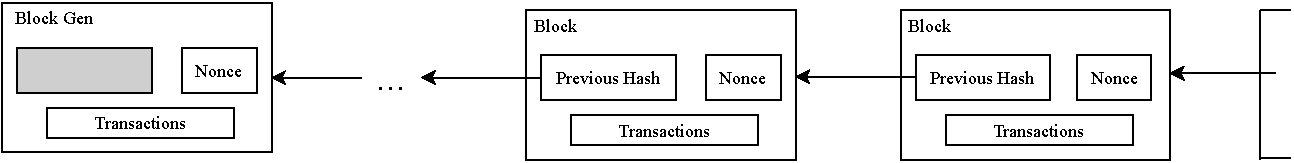
\includegraphics[scale=0.7]{figures/abstract_chain.pdf}
	\end{center}
	\caption{\textit{A high-level representation of a blockchain. }}
	\label{fig:abstract_chain}
\end{figure}


Consider a peer-to-peer network where each party may have one of the following three roles:
lightweight \textit{clients}, full \textit{nodes} and \textit{miners}.
Miners maintain an updated copy of the chain locally, while providing computational power, also
called hashpower, to extend it. In order to extend the chain by one block, the miner has to perform
a proof-of-work as already described.
Full nodes can be thought of as miners with zero hashpower. Full nodes are also called
\textit{provers}, since they provide proofs  answering the queries for specific chain information
made by lightweight clients, according to Simplified Payment Verification (SPV) described by
Nakamoto\cite{Nakamoto}.

According to SPV scheme lightweight clients only need to store the block headers of the longest
valid chain. A block header includes only a Merkle Tree Root of the Merkle Tree comprised by
the transactions included in that specific block. In order to validate that a transaction is
finalized, a client needs to query the nodes until he is convinced that he has the longest
valid chain, search for the block containing that transaction and finally verify an inclusion
proof of the transaction in the block of interest.

\begin{figure}[h!]
	\begin{center}
		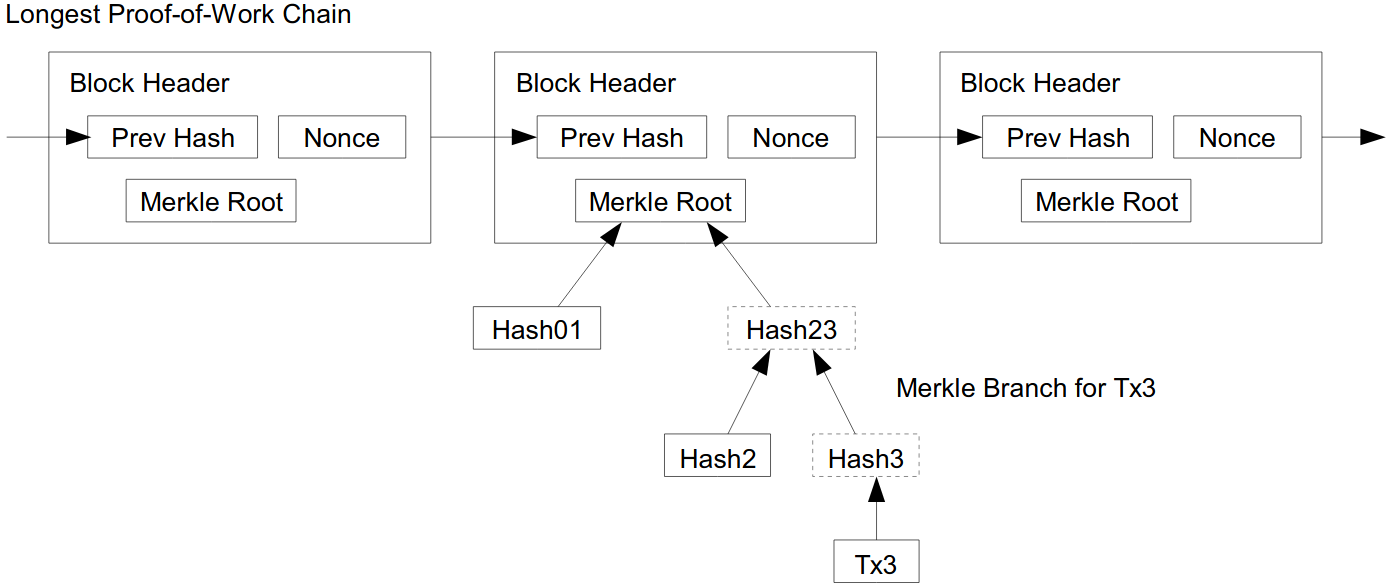
\includegraphics[scale=0.3]{figures/SPV_nakamoto.png}
	\end{center}
	\caption{\textit{ High level representation of blockchain data kept by a lightweight client
	 and an inclusion proof for a transaction Tx3.\cite{Nakamoto}  }}
	\label{fig:SPV_nakamoto}
\end{figure}

In the SPV scheme a client needs to store blockchain data of linear size to the whole chain. By
the time of writing Bitcoin's blockchain counts to almost 264GB and is estimated to grow more
than 50GB per year.  Since the growth rate of the chain is rather linear and constant, we need
to construct more efficient protocols serving the needs of lightweight clients. To this end,
the interaction between lightweight clients and full nodes is in our case supported  by the
NIPoPoWs\cite{NIPoPoWs} primitive which allows polylogarithmic poofs to the size of the chain.

\subsection{The Backbone Model}
The Backbone protocol is executed by an arbitrary number of parties over an unauthenticated network.
We consider $n$ parties in total, $t$ of which may be controlled by an adversary.

Table \ref{table:backbone_parameters} contains all the parameters of the Backbone protocol and will
be a point of reference throughout this work.

\begin{table}[h!]
	\begin{tabular}{| p{14.74cm} |}
		\hline
		$\lambda : \text{security parameter}$\\
		$\kappa : \text{length of the hash function output}$\\
		$n : \text{number of parties mining, } t \text{ of which are controlled by the adversary}$\\
		$T : \text{the target hash value used by parties for solving POW}$\\
		$t :  \text{number of parties controlled by the adversary}$\\
		$\delta : \text{advantage of honest parties}, \dfrac{t}{n-t} \leq 1-\delta$\\
		$f : \text{probability at least one honest party succeeds in finding a POW in a round}$\\
		$\epsilon : \text{random variables' quality of concentration in typical executions}$\\
		$k : \text{number of (suffix) blocks for the common prefix property}$\\
		% be more specific in l please\\
		$l : \text{number of blocks for the chain quality property}$\\
		$\mu_Q : \text{chain quality parameter}$\\
		%% more specific for s too please
		$s : \text{number of rounds for the chain growth property}$\\
		$\tau : \text{chain growth parameter}$\\
		$L : \text{the total run-tiem of the system}$\\
		\hline
	\end{tabular}
	\caption{The parameters of backbone model analysis. Positive integers $n, t, L, s, l, T, k,
	 \kappa$, positive reals $f, \epsilon, \delta, \mu_Q, \tau, \lambda$ where
	 $f, \epsilon, \delta, \mu_Q \in (0,1)$.}
	\label{table:backbone_parameters}
\end{table}

We will now give a high-level description of the Backbone Protocol and its fundamental components,
namely the three supporting algorithms for \textit{chain validation}, \textit{chain comparison} and
\textit{proof of work}. We will also define and discuss the three properties of the protocol, namely
\textit{Common Prefix}, \textit{Chain Quality} and \textit{Chain Growth}. For a more formal and
detailed presentation refer to the Backbone paper\cite{Backbone}.

Consider that the protocol has already run for some rounds and a chain $C$ has been formed. Consider
also an honest party that wishes to connect to the network, obtain the up-to-date version of the
chain and try to extend it.
The honest party connects to the network and first tries to synchronize to the current chain. The
chain synchronization takes two steps to conclude. First, the newly connected peer receives a number
of candidate chains by other peers in the network and validates them one by one as for the structural 
properties of each block \textit{(Chain Validation)}. In particular, for each block the chain
validation algorithm checks that the proof-of-work is properly solved, that the hash of the previous
block is properly included in the block and that the the rest of the information included satisfies
a certain validity predicate $V(\cdot)$ depending on the application. For example, in Bitcoin
application it is checked that all the included transactions are valid according to the
UTXO set.

Afterwards, the \textit{Chain Comparison} algorithm is applied, where all the valid chains are
compared to each other and the longest one, as for total number of blocks or total hashing power
included, is considered the current active chain.

At last, in order to expand the chain by appending one more block to it, the \textit{Proof Of Work}
algorithm is applied, where the miner attempts to solve a proof of work as follows. The miner
constructs the contents of the block, including the hash of the previous block and a number of new
transactions published to the network. Consider that he can calculate the value $h = G(s,x)$ up
to this point. Finally it remains to compute the \textit{ctr} value so that $H(ctr, h) < T$. The
protocol is running in rounds and each party can make at most $q$ queries to function $H(\cdot)$
within a single round. If a suitable \textit{ctr} is found, an honest party quits any queries
remaining and announces the new born block to the network.

We can now define the three desired properties of the backbone protocol.\\
\begin{defn}{\textbf{Common Prefix Property}}
	\textit{The common prefix property $Q_{cp}$ with parameter
$k \in \mathbb{N}$ states that for any pair of honest players $P_1, P_2$ adopting the chains
$C_1, C_2$ at rounds $r_1 \leq r_2$ respectively, it holds that $C_1^{\lceil k} \preceq C_2$.}
	\label{defn:common_prefix}
\end{defn}

\begin{defn}{\textbf{Chain Quality Property}}
	\textit{The chain quality property $Q_{cq}$ with
parameters $\mu_{cq} \in \mathbb{R}$ and $l \in \mathbb{N}$ states that for any honest
party \textit{P} with chain \textit{C}, it holds that for any $l$ consecutive
blocks of \textit{C} the ratio of honest blocks is at least $\mu_{cq}$.}
	\label{defn:chain_quality}
\end{defn}

\begin{defn}{\textbf{Chain Growth Property}}
	\textit{The chain growth property $Q_{cg}$ with
parameters $\tau \in \mathbb{R}$ and $s \in \mathbb{N}$ states that for any honest party
\textit{P} with chain \textit{C}, it holds that for any $s$ rounds there are at least 
$\tau \cdot s$ blocks added to the chain of \textit{P}}
	\label{defn:chain_growth}
\end{defn}

\subsection{NIPoPoWs Preliminaries}

\subsection{Hard, Soft and Velvet Forks}
We typically describe the two common types of a blockchain permanent fork as follows.

A \textit{hard fork} is a consensus protocol upgrade which is not backwards
compatible. This means that the changes in the protocol break the old rules
since the block header's contents change. After a hard fork blocks generated
by upgraded players are not accepted by the unupgraded ones. In order the
protocol update to be well established, the majority of the players must be
upgraded at an early point or else the non-upgraded players may maintain the
longest chain under the old rules.

A \textit{soft fork} is a consensus protocol upgrade which is backwards compatible.
This is usually implemented by keeping the old rules while adding additional
information in a way that unupgraded players can ignore as comments, for example,
by adding adding data in the coinbase transaction. In this way unupgraded players
accept blocks generated by upgraded miners as valid, while, typically, unupgraded
blocks are not accepted by upgraded players. Players are motivated to upgrade in
order their blocks to be accepted in the chain as valid.

A \textit{velvet fork} is also a backwards compatible consensus protocol upgrade.
Similar to soft fork additional data can be inserted in the coinbase transaction.
A velvet fork requires any block compliant to the old protocol rules only to be
accepted as valid by both unupgraded and upgraded players. By requiring upgraded
miners to accept all blocks, even if they contain false data according to the new
protocol rules, we do not modify the set of accepted blocks. Therefore, the upgrade
is rather a \textit{recommendation} and not an actual change of the consensus
protocol.  In reality, the blockchain is never forked. Only the codebase is
upgraded and the data on the blockchain is interpreted differently\cite{NIPoPoWs}.


The goal of this work is to provide a modified NIPoPoWs protocol so that it can be
deployed under a velvet fork in a provably secure manner.
\section{NIPoPoWs under Soft or Hard Fork}
\import{sections/nipopows_hard_fork/}{nipopows_hard_fork.tex}

\section{NIPoPoWs under Velvet Fork}
\import{sections/nipopows_velvet_fork/}{nipopows_velvet_fork.tex}


\subsubsection{Security of Suffix Proofs}
\import{sections/nipopows_velvet_fork/}{suffix_security.tex}


\subsection{Infix Proofs}
The security of the original NIPoPoWs protocol suffers under velvet fork conditions for the case of
infix proofs as well. Again, since blocks containing incorrect interlink pointers are accepted in the 
chain, the adversary may create an infix proof for a transaction included in a block mined on a
different chain. This attack is presented in detail in the following.

An infix proof attack when applying the original protocol under a velvet fork should be obvious
after our previous discussion. So consider the updated protocol for secure suffix proofs as
described in the previous section. A problem here is that in the updated protocol some blocks
are excluded from the interlink, while we should still be able to provide proofs for transactions
included in any block of the chain.

For this reason, let us initially consider an additional protocol patch suggesting to include
a second interlink data structure in each block, which will be updated without any block exclusion,
just as described in the original protocol and will be used for constructing infix proofs only. In
order to be secure we could think of allowing using pointers of the second interlink only for the
\textit{followDown} part of the algorithm. But still, the adversary may use an invalid pointer of a
block visited during the \textit{followDown} procedure and jump to a block of another chain providing 
a transaction inclusion proof concerning that block. This attack is illustrated in
Figure \ref{fig:infix_attack}.

\begin{figure}[h!]
	\begin{center}
		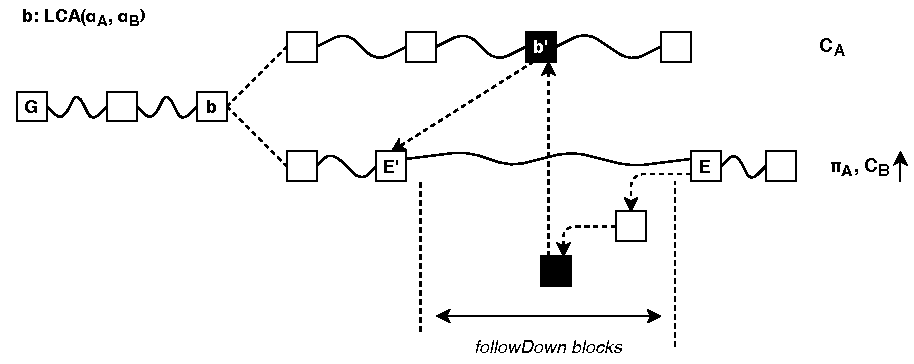
\includegraphics[scale=0.75]{figures/infix_attack.pdf}
	\end{center}
	\caption{\textit{Adversarial fork chain $C_A$ and an adversarial infix proof based on the chain
	 adopted by an honest player. Wavy lines imply one or more blocks. Blocks generated by the
	 adversary are colored black. Dashed arrows represent interlink pointers included in the proof
	 as part of the \textit{followDown} procedure. The adversary provides infix proof for a
	 transaction in block b'. }}
	\label{fig:infix_attack}
\end{figure}

Thus giving the ability to utilize invalid pointers even in a narrow block window can break the
security of our protocol. 

\subsubsection*{Protocol patch for NIPoPoWs infix proofs under velvet fork}
However, since we have proved the security of suffix proofs we can include some more information
in the blocks participating in these proofs in order to provide secure infix proofs as well.
 
Specifically, we suggest full nodes to maintain an authenticated data structure, let's say a
Merkle Tree, for the blocks consisting the longest valid chain at each time point, and each
block to additionally contain the Merkle Tree Root of  the blocks' Merkle Tree. In this way an
infix proof will consist of a suffix proof in order to obtain the longest valid chain and a
block inclusion proof for the block of interest.

For example, in order to prove that a specific transaction $tx_1$ took place in a block $b'$,
the Prover provides:
\begin{itemize}
\item a suffix proof $\pi$
\item a block inclusion proof for $b'$, using the blocks' MTR existing in the tip of the
suffix proof chain $\pi[-1]$
\item a transaction inclusion proof for $tx_1$ using the transactions' MTR of block $b'$
\end{itemize}


The problem with this infix proof construction is that in order to confirm a
transaction in a block of interest $b$ the prover has to provide an inclusion
proof for that block of interest using the Merkle Tree Root of a more recent
honestly generated block included in the infix proof. Obviously, there is a case
that there may be a number of consecutive adversarially generated blocks in the
chain   consisting the prefix of the chain. Thus, no inclusion proof can be provided
for any of these blocks until an honestly generated block is added in the chain and,
consequently in the infix proof.

We need to estimate an upper bound for the number of rounds a client has to
wait until the block of interest is buried under sufficient number of blocks
so that he can obtain the infix proof needed with high probability.

Consider $n_b$ is the upper bound on the consecutive rounds when the adversary could
possibly append blocks to the chain, without any honestly generated blocks in
between. The adversary mines either by following the selfish mining strategy or
not. The state of the chain we examine looks like in Figure \ref{fig:infix_delay}.

\begin{figure}[h!]
	\begin{center}
		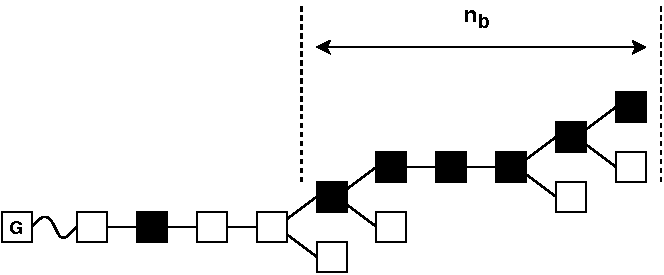
\includegraphics[scale=0.75]{figures/infix_delay.pdf}
	\end{center}
	\caption{\textit{Wavy lines imply one or more blocks. Blocks generated by the
	 adversary are colored black. \textbf{$n_b$} implies the number of consecutive
	 adversarially generated blocks in the chain.}}
	\label{fig:infix_delay}
\end{figure}

Let $p_H$ the probability that a block is generated by an honest party during a round.
Then considering that collisions in RO model is a negligible event we have
$p_H = (n-t)qp$. Let $p_A$ be the probability that a block is generated by the
adversary during a round, then $p_A = tqp$. Consider $N_{bA}$ the random variable
for the number of consecutive blocks generated by the adversary in a total of $r$
rounds. Also let $N_{bH}$ the random variable for the number of blocks generated by
honest parties in total of $r$ rounds. 
Then we have that $N_{bA}$, $N_{bH}$ follow the Binomial Distribution with
probability $p_A$, $p_H$ respectively.

Because we require consecutive successful rounds for the adversary, we have:
\begin{equation}
	Pr[N_{bA} = n_b] = (r-n_b - 1) p_A^{n_b}(1-p_A)^{r-n_b}
\end{equation}

while for the honest players we have 
\begin{equation}
	Pr[N_{bH} \leq n_b] = \sum_{i=0}^{n_b} \binom nk p_H^{i}(1-p_H)^{r-i}
\end{equation}

If $N_b$ is the random variable denoting the number of consecutive rounds that
adversarially generated blocks are appended to the chain, we have:

\begin{equation}
	Pr[N_b = n_b] = Pr[N_{bA} = n_b] \cdot Pr[N_{bH} \leq n_b]
\end{equation}

since the two events are independent.

\subsubsection*{The velvet infix prover}
The construction of an infix proof is described in Algorithm \ref{alg:proveInfixVelvet}. In order
to keep the algorithm generic enough for any infix-sensitive predicate, we provide the steps
needed until the verification of the block of interest and consider the specific predicate answer
as trivial to calculate given the block of interest. The infix prover accepts as input the full
chain $C$ and a block of interest $b'$ and returns a proof consisting of the Merkle Tree proof
of inclusion for $b'$ and a suffix proof.
\vspace{4mm}

\begin{algorithm}[H]
\SetAlgoNoLine
\DontPrintSemicolon
\SetKwProg{Fn}{function}{:}{\text{end function}}
\Fn{ProveInfixVelvet(C, b')}{
	$(\pi , \chi) \leftarrow Prove_{m,k}(C)$\;
	$tip = \pi [-1]$\;
	$\pi_{b'} \leftarrow \text{ConstrMTInclProof}(tip, b'.id )$\;
 
 
 	\Return ($\pi_b', (\pi, \chi)$)\;
}
 \caption{Velvet Infix Prover}
 \label{alg:proveInfixVelvet}
\end{algorithm}

\vspace{4mm}

\subsubsection*{The velvet infix verifier}
The infix proof verification algorithm is described in Algorithm \ref{alg:verifyInfixVelvet}.
Supposing that the verifier has already concluded to the longest valid chain $C$ after accepting
and comparing constesting suffix proofs, the infix verification algorithm only has to confirm
the Merkle-Tree inclusion proof for the block of interest $b'$.

\vspace{4mm}

\begin{algorithm}[H]
\SetAlgoNoLine
\DontPrintSemicolon
\SetKwProg{Fn}{function}{:}{\text{end function}}
\Fn{VerifyInfixVelvet($\pi_b', (\pi, \chi)$)}{
	$(\pi , \chi) \leftarrow Prove_{m,k}(C)$\;
	$tip = \pi [-1]$\;
	\Return $\text{VerMTInclProof}(tip.MTR_{blocks}, \pi_{b'}, b'.id )$\;
}
 \caption{Velvet Infix Verifier}
 \label{alg:verifyInfixVelvet}
\end{algorithm}

\vspace{4mm}

\bibliographystyle{plain} % We choose the "plain" reference style
\bibliography{refs} % Entries are in the "refs.bib" file

\end{document}